\documentclass[12pt]{article}
%\setlength{\oddsidemargin}{0in}
%\setlength{\topmargin}{0.0in}
%\setlength{\textwidth}{6.7in}
%\setlength{\textheight}{8.5in}
%
\usepackage{graphicx}
\usepackage{enumitem}
\usepackage{mathtools}
\usepackage[usenames,dvipsnames]{xcolor}

\usepackage{geometry}
 \geometry{
 letterpaper,
 textwidth=6.5in
 }
\usepackage[utf8]{inputenc}
%\usepackage{libertine}
%\usepackage{libertinust1math}
\usepackage[libertine,cmintegrals,cmbraces,vvarbb]{newtxmath}
%\usepackage{newtxmath}
%\usepackage[osf]{ebgaramond}
\usepackage[T1]{fontenc}
%\usepackage{palatino}
\usepackage{microtype}

\usepackage{fancyhdr}
%\usepackage[colorlinks=true]{hyperref}

\pagestyle{fancy}
\fancyhf{}
\fancyhead[RE,LO]{\textcolor{BlueViolet}{Vibrations and Waves}}
\fancyhead[LE,RO]{ph2a: 2017}
\fancyfoot[RE,LO]{\textcolor{Orange}{Caltech}}
\fancyfoot[LE,RO]{\textcolor{Orange}{Physics, Math, and Astronomy}}

%\input mydefs.tex
\def\vev#1{\left\langle #1\right\rangle}
\def\hb{\hfill\break}
%
\begin{document}
%
\begin{centering}
\LARGE{QP 8: LIDAR by Interference}
\end{centering}
\bigskip
\bigskip

NASA would like to improve its ability to sense atmospheric CO$_2$ and
CH$_4$. To
that end we need to design a sensitive phased array of lasers to
perform light detection and ranging (LIDAR).

\begin{figure}[!h]
  \centering
    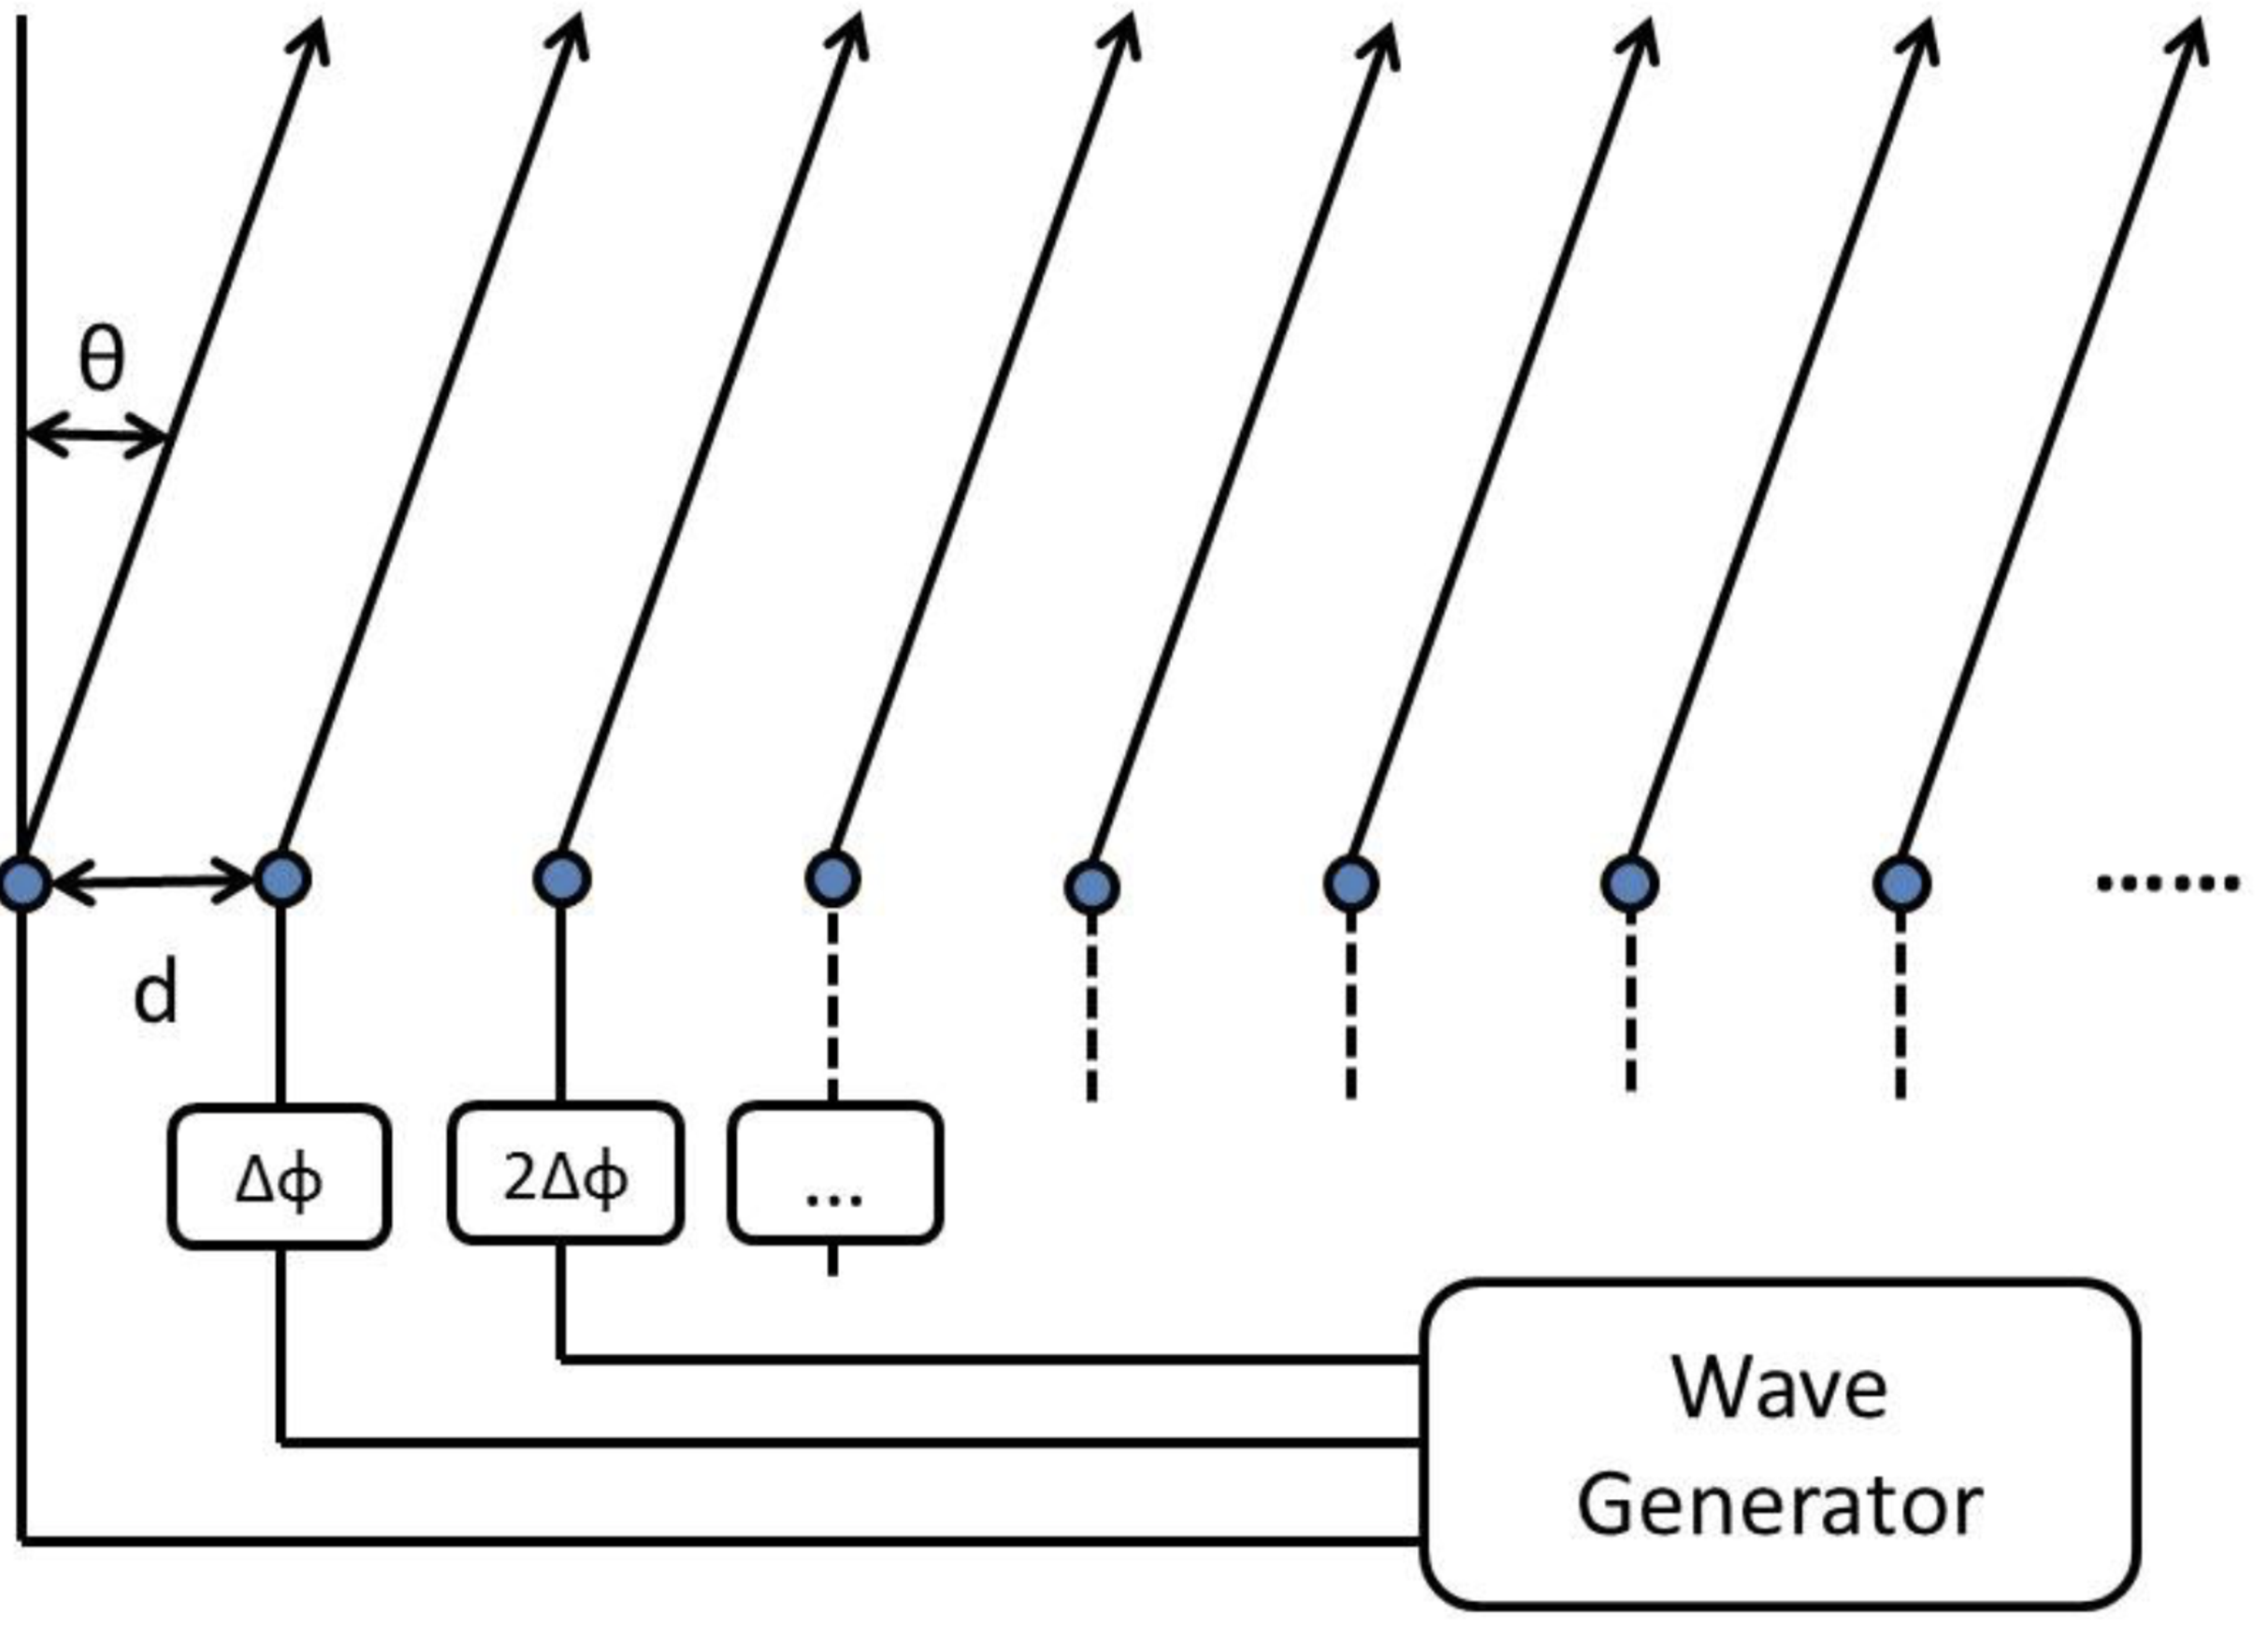
\includegraphics[width=0.42\textwidth]{PhasedArray.pdf}
    %\caption{}
\end{figure}
Each laser, denoted as a small circle, is separated from the
adjacent one by some distance $d$. The array is then connected to a wave
generator that is configured to control the \emph{phase} of each
laser. When the generator is turned on, each antenna acts as a
wave source and emits EM waves of the same wavelength, $\lambda$. 
A beam can be ``directed'' to a certain direction by manipulating the
relative phase shift among the lasers without moving the array itself.

\begin{enumerate}[label=(\alph*)]
\item (5 pts)
Determine the relative phase delay $\Delta \phi$ between the adjacent
lasers required to steer the beam at an angle $\theta$. Express your
answer 
in terms of $d$, $\theta$, and $\lambda$.

\item (5 pts)
Using the phase delay computed in (a), is $\theta$ the only angle at which
radio beams are directed? If not, find the other angles 
in terms of $d$, $\theta$, and $\lambda$.

\item (5 point)
Our laser array is mounted on board a satellite which is orbiting the
Earth. The beam reflects off the side of a mountain and gets reflected
back to the array. Assume that the velocity of the mountain with
respect to the array is $v$ in the $\theta$ direction and that the
speed of light in air is $c$ (same as in vacuum). 
What is the frequency difference between the emitted and reflected light?

\item (5 pts)
Suppose now that you also have a phased array of receivers on the same
satellite. How should you configure the phase of the receivers so as
to maximize the signal reflected from the mountain?
Assume that the mountain is very far away, so that the waves you 
receive at the satellite
can be approximated by plane waves incident at the same angle $\theta$.

\end{enumerate}
\bigskip


{\color{Sepia} \hrule}







\end{document}
